Given a batch update on the original graph, it is likely that only a small subset of vertices in the graph would change their community membership. Selection of the appropriate set of affected vertices to be processed (that are likely to change their community), in addition to the overhead of finding them, plays a significant role in the overall accuracy and efficiency of a dynamic batch parallel algorithm. Too small a subset may result in poor-quality communities, while a too-large subset will increase computation time. However, the Naive-dynamic (ND) approach processes all the vertices, while the Delta-screening (DS) approach generally overestimates the set of affected vertices and has a high overhead. Our proposed Dynamic Frontier (DF) approach addresses these issues.




\subsection{Our Dynamic Frontier (DF) approach}
\label{sec:frontier}

We now explain the \textit{Dynamic Frontier} approach. Consider a batch update consisting of edge deletions $(i, j, w) \in \Delta^{t-}$ and insertions $(i, j, w) \in \Delta^{t+}$, both shown with dotted lines, with respect to a single source vertex $i$, in Figure \ref{fig:about-cases--frontier}. At the start of the community detection algorithm, we initialize the community membership of each vertex to that obtained in the previous snapshot of the graph.

\begin{figure*}[hbtp]
  \centering
  \subfigure[Naive-dynamic (ND) approach]{
    \label{fig:about-cases--naive}
    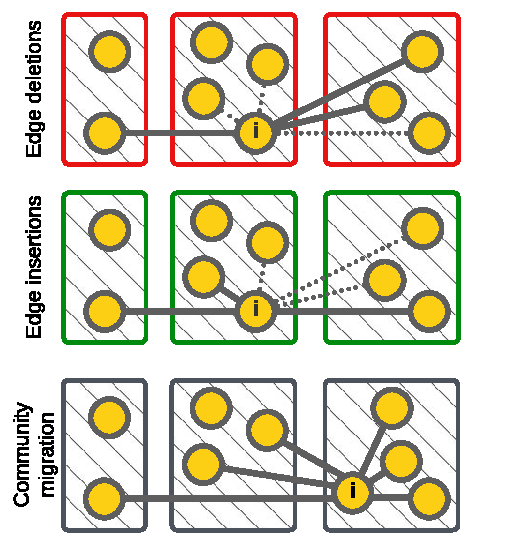
\includegraphics[width=0.3\linewidth]{out/about-cases-naive.pdf}
  }
  \subfigure[Delta-screening (DS) approach]{
    \label{fig:about-cases--delta}
    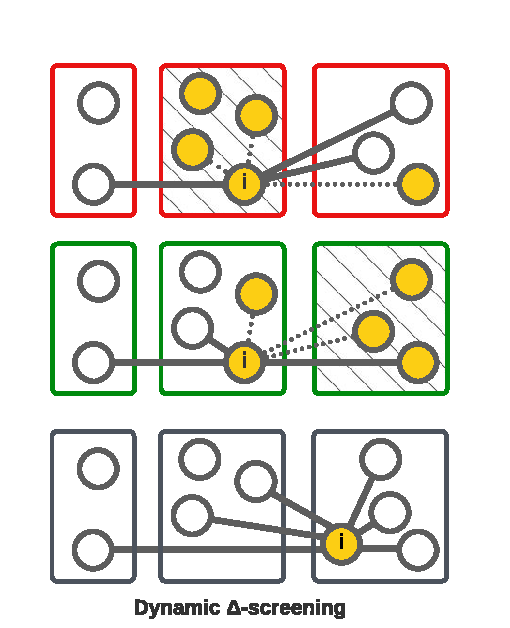
\includegraphics[width=0.3\linewidth]{out/about-cases-delta.pdf}
  }
  \subfigure[Dynamic Frontier (DF) approach]{
    \label{fig:about-cases--frontier}
    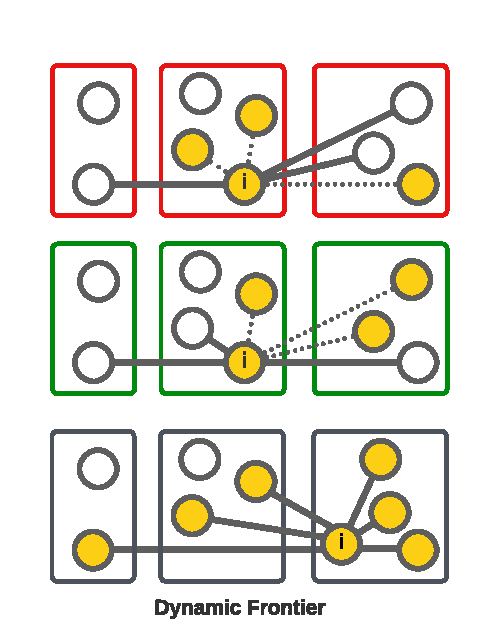
\includegraphics[width=0.3\linewidth]{out/about-cases-frontier.pdf}
  } \\[-2ex]
  \caption{Comparison of dynamic community detection approaches: \textit{Naive-dynamic (ND)}, \textit{Delta-screening (DS)}, and our \textit{Dynamic Frontier (DF)} approach. Edge deletions/insertions are indicated with dotted lines. Vertices marked as affected (initially) with each approach are highlighted in yellow, and when entire communities are marked as affected, they are hatched.}
  \label{fig:about-cases}
\end{figure*}

\begin{figure*}[!hbtp]
  \centering
  \subfigure[]{
    \label{fig:frontier-example-01}
    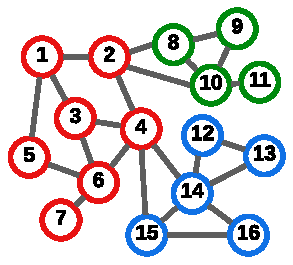
\includegraphics[width=0.18\linewidth]{out/about-frontier-01.pdf}
  }
  % \subfigure{
  %   \label{fig:frontier-example-02}
  %   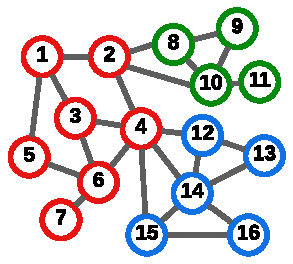
\includegraphics[width=0.15\linewidth]{out/about-frontier-02.pdf}
  % }
  \subfigure[]{
    \label{fig:frontier-example-03}
    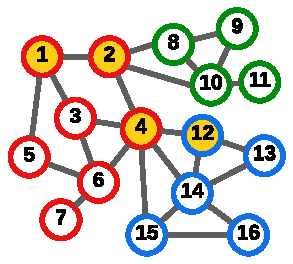
\includegraphics[width=0.18\linewidth]{out/about-frontier-03.pdf}
  }
  \subfigure[]{
    \label{fig:frontier-example-04}
    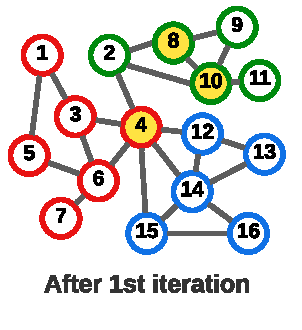
\includegraphics[width=0.18\linewidth]{out/about-frontier-04.pdf}
  }
  \subfigure[]{
    \label{fig:frontier-example-05}
    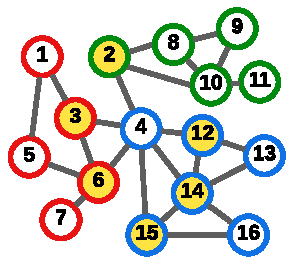
\includegraphics[width=0.18\linewidth]{out/about-frontier-05.pdf}
  }
  \subfigure[]{
    \label{fig:frontier-example-06}
    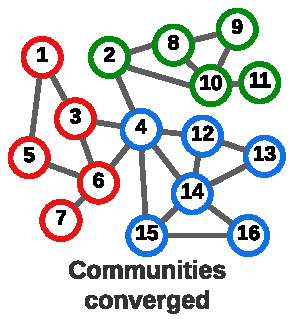
\includegraphics[width=0.18\linewidth]{out/about-frontier-06.pdf}
  } \\[-2ex]
  \caption{An example explaining the \textit{Dynamic Frontier} approach (\Fro{}). The community membership of each vertex is shown with border color (red, green, or blue), and the algorithm proceeds from left to right. A batch update arrives, affecting vertices $1$, $2$, $4$, and $12$. In the first iteration, vertex $2$ switches from red to green, impacting neighbors $8$ and $10$. In the second iteration, vertex $4$ changes from red to blue, affecting neighbors $3$, $6$, $12$, $14$, and $15$. Afterward, there are no more community changes.}
  % An example explaining the \textit{Dynamic Frontier} approach (\Fro{}). The community membership of each vertex is shown with border color (red, green, or blue), and the algorithm proceeds from left to right. \su{A batch update arrives, consisting of $\Delta^{t-}=\{(1, 2)\}$ and $\Delta^{t+}=\{(4, 12)\}$. Initially, \Fro{} marks vertices $1$, $2$, $4$, and $12$ as affected. In the first iteration, $2$ changes its membership from \textit{red} to \textit{green}, affecting neighbors $8$ and $10$. In the second iteration, $4$ changes its community from \textit{red} to \textit{blue}, affecting neighbors $3$, $6$, $12$, $14$, and $15$. Subsequently, no further community changes occur.
  \label{fig:frontier-example}
\end{figure*}


\paragraph{Initial marking of affected vertices upon edge deletion/insertion}

For edge deletions between vertices belonging to the same community and edge insertions between vertices belonging to different communities, we mark the source vertex $i$ as affected, as shown with vertices highlighted in yellow, in Figure \ref{fig:about-cases--frontier}. Note that batch updates are undirected, so we effectively mark both the endpoints $i$ and $j$. Edge deletions between vertices lying across communities and edge insertions for vertices lying within the same community are ignored (for reasons stated before, in Section \ref{sec:delta-screening}).

\paragraph{Incremental marking of affected vertices on vertex migration to another community}

When a vertex $i$ changes its community during the community detection algorithm (shown by moving $i$ from its original community in the center to its new community on the right), we mark all its neighbor vertices $j \in J_i$ as affected, as shown in Figure \ref{fig:about-cases--frontier} (highlighted in yellow), and mark $i$ as not affected. If $i$ does not change its community, it is also marked as unaffected --- this is known as vertex pruning optimization \cite{com-ozaki16, com-ryu16, com-shi21, com-zhang21}. The process is akin to a graph traversal and continues until the community assignments of the vertices have converged.

\paragraph{Application to the first pass of Louvain algorithm}

We apply the DF approach to the first pass of Louvain algorithm\ignore{(see line \ref{alg:louvain--remark-pass} in Algorithm \ref{alg:louvain})}, as with the DS approach. In subsequent passes\ignore{, if the aggregation tolerance condition is not met (line \ref{alg:louvain--aggregation-tolerance} in Algorithm \ref{alg:louvain}),} all super-vertices are\ignore{marked as affected and} processed, according to the Louvain algorithm. This takes less than $15\%$ of total time, on average, so we don't use the DF approach to find affected super-vertices.\ignore{The tolerance condition only fails in the case of large batch updates.} The psuedocode for our parallel DF Louvain is given in Algorithm \ref{alg:frontier}, with its explanation in Section \ref{sec:our-frontier}. Similar to our parallel ND/DS Louvain, it utilizes\ignore{weighted-degrees of vertices and total edge weights of communities as} auxiliary information.


\subsubsection{An example of DF approach}

See Figure \ref{fig:frontier-example}\ignore{shows an example of our DF approach}.

\paragraph{Initial communities}

The original graph consists of $16$ vertices, which are divided into three communities, distinguished by the border colors of \textit{red}, \textit{green}, and \textit{blue} (see Figure \ref{fig:frontier-example-01}). This community membership\ignore{information} of each vertex could have been obtained by executing either the static or dynamic version of Louvain algorithm.

\paragraph{Batch update and marking affected (initial)}

Subsequently a batch update is applied to the original graph (see Figure \ref{fig:frontier-example-03}), involving and edge deletion between vertices $1$ and $2$, and an insertion vertices $4$ and $12$. Following the batch update, we perform the initial step of the DF approach, marking endpoints $1$, $2$, $4$, and $12$ as affected. Now, we are ready to execute the first iteration of Louvain algorithm.

\paragraph{After first iteration}

During the first iteration (see Figure \ref{fig:frontier-example-04}), the community membership of vertex $2$ changes from \textit{red} to \textit{green} because it exhibits stronger connections with vertices in the \textit{green} community. In response to this change, the DF approach incrementally marks the neighboring vertices of $2$ as affected, specifically vertices $8$ and $10$. Vertex $2$ is no longer\ignore{marked as} affected due to pruning.

\paragraph{After second iteration}

Let us now consider the second iteration (see Figure \ref{fig:frontier-example-05}). Vertex $4$ is now more strongly connected to the \textit{blue} community, resulting in a change of its community membership from \textit{red} to \textit{blue}. As before, we mark the neighbors of vertex $4$ as affected, namely vertices $12$, $14$, and $15$. Vertex $4$, once again, no longer marked as affected due to vertex pruning.

\paragraph{Communities converged}

In the subsequent iteration (see Figure \ref{fig:frontier-example-06}), no other vertices have a strong enough reason to change their community membership. At this point\ignore{, when employing the Louvain algorithm}, the aggregation phase commences, consolidating communities into super-vertices to prepare for the subsequent pass of Louvain algorithm.




\subsection{Utilizing Auxiliary information}
\label{sec:auxiliary}

We note that computing the weighted-degree of each vertex $K^t$ and the total edge weight of each community $\Sigma^t$ incurs considerable runtime, in comparison to the time required for the local-moving and aggregation phases of the Louvain algorithm\ignore{to converge, especially for small batch updates}. It would be more efficient to incrementally update the previous weighted-degrees of vertices $K^{t-1}$ and total edge weights of communities $\Sigma^{t-1}$ by taking into account edge deletions $\Delta^{t-}$ and insertions $\Delta^{t+}$ within the batch update, instead of recomputing from scratch. We refer to $K^t$ and $\Sigma^t$ (and $K^{t-1}$, $\Sigma^{t-1}$) as auxiliary information as they must be maintained by the dynamic algorithm, but do not represent the output of the algorithm. Figure \ref{fig:about-auxiliary} illustrates this concept.

In Figure \ref{fig:adjust-auxiliary}, we present the mean speedup observed for ND, DS, and DF Louvain when making use of auxiliary information $K^{t-1}$ and $\Sigma^{t-1}$, in contrast to the same dynamic algorithm when calculating from scratch. This is done on graphs from Table \ref{tab:dataset-large} with random batch updates of size $10^{-7} |E|$ to $0.1 |E|$, consisting of $80\%$ edge insertions and $20\%$ edge deletions, to simulate realistic dynamic graph updates. Results indicate that employing auxiliary information enables ND, DS, and DF Louvain to achieve average speedups of $11.8\times$, $2.9\times$, and $48.5\times$, respectively. Moreover, DF Louvain achieves remarkable speedups, reaching up to $107\times$ for smaller batch sizes. Incrementally updating $K^{t-1}$ and $\Sigma^{t-1}$ to obtain $K^t$ and $\Sigma^t$, thus, significantly speeds up DF Louvain. To the best of our knowledge, none of the existing dynamic algorithms for Louvain algorithm make such use of auxiliary information.

\begin{figure}[hbtp]
  \centering
  % \subfigure[Without using auxiliary information]{
  %   \label{fig:about-auxiliary--without}
  %   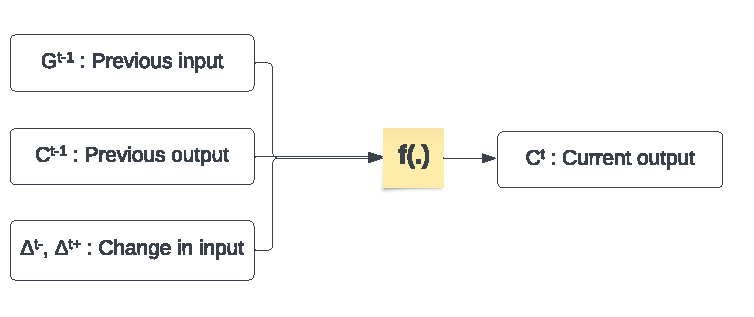
\includegraphics[width=0.48\linewidth]{out/about-auxiliary-without.pdf}
  % }
  \subfigure{
    \label{fig:about-auxiliary--with}
    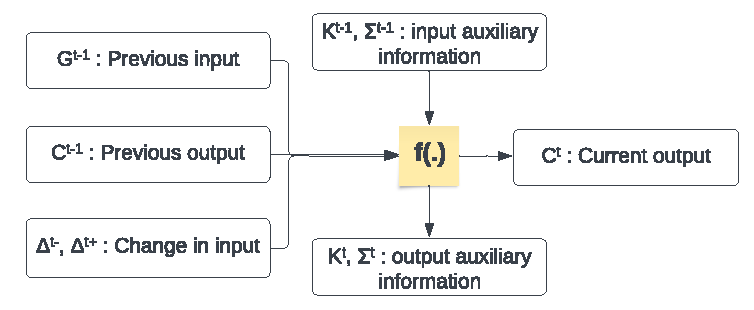
\includegraphics[width=0.98\linewidth]{out/about-auxiliary-with.pdf}
  } \\[-2ex]
  \caption{A dynamic community detection algorithm $f(.)$ accepts as input the previous graph $G^{t-1}$, community memberships $C^{t-1}$, and the batch update $\Delta^{t-}$, $\Delta^{t+}$, and returns the updated community memberships $C^t$. However\ignore{, as shown in (b)}, it may also accept weighted degree of vertices $K^{t-1}$ and total edge weights of communities $\Sigma^{t-1}$ as auxiliary information, and generate updated auxiliary information $K^t$, $\Sigma^t$.}
  \label{fig:about-auxiliary}
\end{figure}

\begin{figure}[hbtp]
  \centering
  \subfigure{
    \label{fig:adjust-auxiliary--8020}
    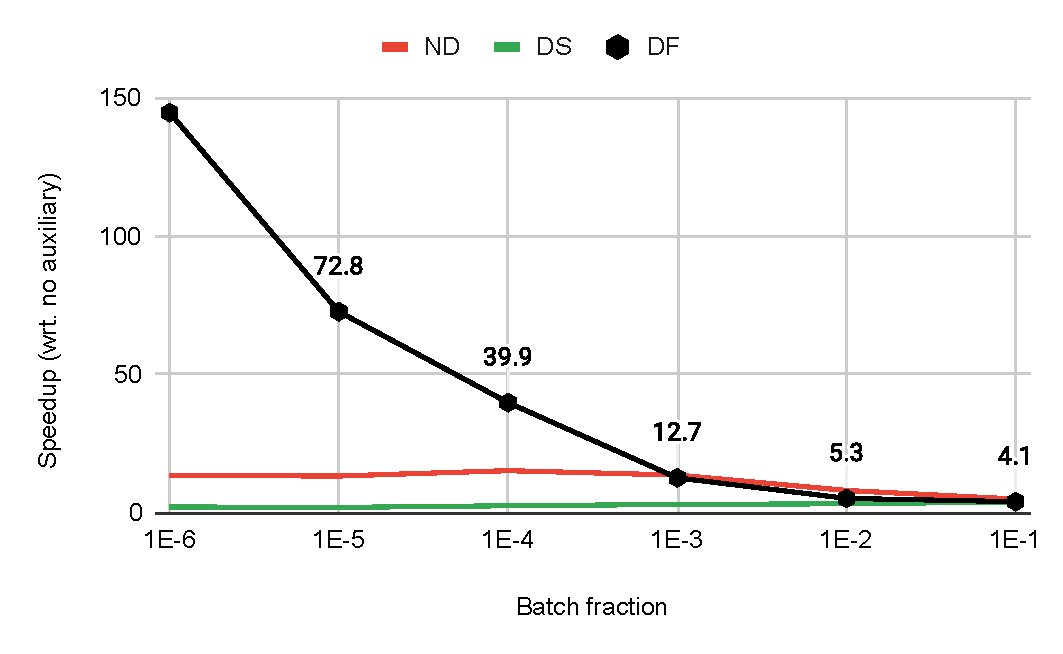
\includegraphics[width=0.98\linewidth]{out/adjust-auxiliary-8020.pdf}
  } \\[-2ex]
  \caption{Speedup of \textit{Naive-dynamic (ND)}, \textit{Delta-screening (DS)}, and \textit{Dynamic Frontier (DF)} Louvain when reusing the previous \textit{weighted-degrees of vertices} and \textit{total edge weight of communities} as auxiliary information to the dynamic algorithm, compared to the same dynamic algorithm when both are recomputed from scratch. This is done on large graphs with generated random batch updates of size $10^{-7} |E|$ to $0.1 |E|$\ignore{, consisting of $80\%$ edge insertions and $20\%$ deletions, to simulate realistic dynamic graph updates}.}
  \label{fig:adjust-auxiliary}
\end{figure}





\subsection{Our DF Louvain implementation}
\label{sec:our-frontier}

Algorithm \ref{alg:frontier} shows the psuedocode of our Parallel Dynamic Frontier (DF) Louvain. It takes as input the previous $G^{t-1}$ and current graph snapshot $G^t$, edge deletions $\Delta^{t-}$ and insertions $\Delta^{t+}$ in the batch update, the previous community assignments $C^{t-1}$ for each vertex, the previous weighted-degrees $K^{t-1}$ of vertices, and the previous total edge weights $\Sigma^{t-1}$ of communities. It returns the updated community memberships $C^t$ of vertices, weighted-degrees $K^t$, and total edge weights $\Sigma^t$ of communities.

\begin{algorithm}[hbtp]
\caption{\textit{Dynamic Frontier} community detection approach.}
\label{alg:frontier}
\begin{algorithmic}[1]
\Ensure{$\delta V[i]$: Is vertex $i$ affected due to current batch update?}
\Ensure{$communities$: Community detection algorithm to use.}

\Statex

\Function{dynamicFrontier}{$G^{t-1}, C^{t-1}, \Delta^{t-}, \Delta^{t+}$}
  \State $G^t \gets (G^{t-1} \setminus \Delta^{t-}) \cup \Delta^{t+}$
  \ForAll{$i \in V^{t-1} \cup V^t$} $\delta V[i] \gets 0$
  \EndFor
  \State $\rhd$ Mark initial affected vertices \label{alg:frontier--mark-begin}
  \ForAll{$(i, j) \in \Delta^{t-}$ \textbf{in parallel}}
    \If{$C^{t-1}[i] = C^{t-1}[j]$} $\delta V[i] \gets 1$
    \EndIf
  \EndFor
  \ForAll{$(i, j, w) \in \Delta^{t+}$ \textbf{in parallel}}
    \If{$C^{t-1}[i] \neq C^{t-1}[j]$} $\delta V[i] \gets 1$
    \EndIf
  \EndFor \label{alg:frontier--mark-end}
  \State \BeginHighlight{} $\rhd$ Called to check if a given vertex is affected \label{alg:frontier--affected-begin}
  \Function{isAffected}{$i$}
    \Return{$\delta V[i]$}
  \EndFunction \label{alg:frontier--affected-end}
  \EndHighlight{blue}{0.95}
  \State \BeginHighlight{} $\rhd$ Called when a vertex changes its community \label{alg:frontier--remark-begin}
  \Function{onChange}{$i$}
    \ForAll{$j \in G^t.out(i)$} $\delta V[j] \gets 1$ \Comment{Expand affected}
    \EndFor
  \EndFunction \label{alg:frontier--remark-end}
  \EndHighlight{red}{0.95}
  \State $\rhd$ Find with $louvain()$, $lpa()$, or $hybridLouvainLpa()$ \label{alg:frontier--communities-begin}
  \Return{$communities(G^t, C^{t-1}, \{isAffected, onChange\})$} \label{alg:frontier--communities-end}
\EndFunction
\end{algorithmic}
\end{algorithm}




%% Parameter setting
% $\tau \gets TOLERANCE\_INITIAL$
% TOLERANCE\_INITIAL = 0.01
% TOLERANCE\_DECLINE = 10
% MAX\_PASSES = 500


In the algorithm, we first identify an initial set of affected vertices, whose communities may directly change due to the batch updates, by marking them in the flag vector $\delta V$. We do this by marking the endpoints of edge deletions $\Delta^{t-}$ which lie in the same community (lines \ref{alg:frontier--loopdel-begin}-\ref{alg:frontier--loopdel-end}), and by marking the endpoints of edge insertions $\Delta^{t+}$ which lie in disjoint communities (lines \ref{alg:frontier--loopins-begin}-\ref{alg:frontier--loopins-end}). We then define three lambda functions for the Louvain algorithm, \texttt{isAffected()} (lines \ref{alg:frontier--isaff-begin}-\ref{alg:frontier--isaff-end}), \texttt{inAffectedRange()} (lines \ref{alg:frontier--isaffrng-begin}-\ref{alg:frontier--isaffrng-end}), and \texttt{onChange()} (lines \ref{alg:frontier--onchg-begin}-\ref{alg:frontier--onchg-end}), which indicate that a set of vertices are (initially) marked as affected, that all vertices in the graph can be incrementally marked as affected, and that the neighbors of a vertex are marked as affected if it changes its community membership, respectively. Note that the set of affected vertices will expand automatically due to vertex pruning optimization used in our Parallel Louvain algorithm (Algorithm \ref{alg:louvain}). Thus, \texttt{onChange()} reflects what the DF approach would do in the absence of vertex pruning. Further, unlike existing approaches, we leverage $K^{t-1}$ and $\Sigma^{t-1}$, alongside the batch updates $\Delta^{t-}$ and $\Delta^{t+}$, to efficiently compute $K^t$ and $\Sigma^t$ required for the local-moving phase of the Louvain algorithm (line \ref{alg:frontier--auxiliary}). These lambda functions and the total vertex/edge weights are then utilized to execute the Louvain algorithm and obtain the updated community assignments $C^t$ (line \ref{alg:frontier--louvain}). Finally, we return $C^t$, alongside $K^t$ and $\Sigma^t$\ignore{, serving as the updated auxiliary information} (line \ref{alg:frontier--return}).




\ignore{\subsection{Time and Space complexity}}
\ignore{\label{sec:complexity}}

\ignore{To discuss the time complexity of DF Louvain, we use $N_B$ to denote the number of vertices marked as affected (which is dependent on the size and nature of batch update) by it on a batch $B$ of edge updates, $M_B$ to denote the number of edges with one endpoint in $N_B$, and $K$ to denote the total number of iterations performed. Then, the time complexity of DF Louvain is $O(K M_B)$.\ignore{In the worst case, the time complexity of our algorithms would be the same as that of the respective static algorithms, i.e., $O(KM)$.} The space complexity of DF Louvain is the same as that of Static Louvain, i.e., $O(N + M)$.}
